\documentclass{article}

\usepackage[final]{nips}

\usepackage[utf8]{inputenc} % allow utf-8 input
\usepackage[T1]{fontenc}    % use 8-bit T1 fonts
\usepackage{hyperref}       % hyperlinks
\usepackage{url}            % simple URL typesetting
\usepackage{booktabs}       % professional-quality tables
\usepackage{amsfonts}       % blackboard math symbols
\usepackage{nicefrac}       % compact symbols for 1/2, etc.
%\usepackage{microtype}      % microtypography
\usepackage{amsmath}
\usepackage{bm}
\usepackage{tikz}
\usetikzlibrary{bayesnet}

\newcounter{question}
\newcommand{\question}{\stepcounter{question}\paragraph{Question \thequestion}}
\newcommand{\mat}[1]{\textbf{\textit{#1}}}

\title{Coursework 1 - Modelling}

\author{
  Jonas Osborn \\
  \texttt{jo14944} \\
  \And
  Tristan Saunders \\
  \texttt{ts16802} \\
  \And
  Corin Varney \\
  \texttt{cv14985} \\
}

\begin{document}

\maketitle

\section{The prior}
\subsection{Theory}
\question \emph{1.} As the instances of $y$ are noisy observations of the underlying process and we do not know anything about this uncertainty we can assume it is the sum of independent and identically distributed errors. The Central Limit Theorem states the distribution of the sum of a large enough number of independent, identically distributed variables will be approximately normally distributed. From this we can say that our model of $y$ has the following form:
\begin{align*}
	y & = f(x) + \epsilon \\
	\text{where:~}
	\epsilon & \sim \mathcal{N}(0, \mat{I})
\end{align*}
And so from this we have the likelihood of each $y_i$ as a Gaussian distribution with mean $f(x_i)$.\\

\emph{2.} Choosing a spherical covariance matrix for the likelihood means that we are assuming the different dimensions of $y_i$ to be independent and identically distributed. As they are independent they do not covary with each other and so the covariance matrix is diagonal. As they are identically distributed they all have the same variance. Therefore the covariance matrix is spherical.
\question
\begin{align*}
	p(\mat{Y}|f,\mat{X}) &= p(\mat{y}_N|\mat{y}_{N-1},\ldots,\mat{y}_1,f,\mat{X})p(\mat{y}_{N-1}|\mat{y}_{N-2},\ldots,\mat{y}_1,f,\mat{X})\ldots p(\mat{y}_1|f,\mat{X}) \\
\end{align*}
\subsubsection{Linear regression}
\question
\begin{align*}
	p(\mat{Y}|\mat{X},\mat{W}) &= \prod_{i}^Np(\mat{y}_i|\mat{x}_i,\mat{W}) \\
	&= \prod_{i}^N\mathcal{N}(\mat{W}\mat{x}_i,\sigma^2\mat{I}) \\
	&= \mathcal{N}(\mat{W}\mat{X},\sigma^2\mat{I})
\end{align*}
\question A conjugate prior is one that is conjugate to the posterior, meaning they are in the same family of distributions. A conjugate prior is useful as it gives a closed-form solution for the posterior. If we didn't choose a conjugate prior then numerical integration may be necessary to calculate the posterior which may mean the solution is potentially intractable. The conjugate prior for a Gaussian posterior is a Gaussian.
\question Just as encoding the prefrence in a $L_2$ norm is equivalent to having a Gaussian prior, encoding the preference using a $L_1$ norm is equivalent to having a Laplace prior. This is because the Laplace distribution estimates median rather than the mean estimated by the Guassian and median minimises the $L_1$ norm and mean the $L_2$

The shape of the laplace distribution's probability density function, with it's higher peak around zero compared to the probability density function of a Gaussian means that more co-efficients are likely to be equal to zero and this leads to a sparser model than those produced by a Gaussian prior.
\question
\begin{align*}
	p(\mat{W}|\mat{X},\mat{Y}) &= \frac{1}{Z}p(\mat{Y}|\mat{X},\mat{W})p(\mat{W}) \\
	&= \frac{1}{Z}\mathcal{N}(\mat{W}\mat{X},\sigma^2\mat{I})\mathcal{N}(\mat{W}_0,\tau^2\mat{I})
\end{align*}
$\frac{1}{Z}$ is a normalising constant to ensure that the posterior is a true probability distribution and so we will ignore the other constants for now as they will be dealt with by $Z$.

By the probability density function of the multivariate normal distribution, we have:
\begin{align*}
	p(\mat{W}|\mat{X},\mat{Y}) &\propto \exp\Big(-\frac{1}{2\sigma^2}(\mat{Y}-\mat{X}\mat{W})^T\mat{I}(\mat{Y}-\mat{X}\mat{W})\Big) \\
	&\quad\times\exp\Big(-\frac{1}{2\tau^2}(\mat{W}-\mat{W}_0)^T\mat{I}(\mat{W}-\mat{W}_0)\Big) \\
	&\propto \text{[TODO]}
\end{align*}
\subsubsection{Non-parametric regression}
\question Parametric models assume that the distribution the data comes from is based on a finite, fixed set of parameters and models future predictions based off these parameters, they capture everything there is to know about the data. Non-parametric models do not make such assumptions about the model structure and instead infer structure from the data, they have parameters but these are not fixed in advance and there can be an infinite set of parameters.

Non-parametric models are more flexible and can represent a wider variety of data and will represent the data better if the assumptions made in the parametric model are incorrect but are less precise and accurate than parametric methods if the right assumptions are made.

Parametric models are often easier interpreted as they are simpler to transcribe and are also often faster to compute due to lacking the complexity and flexibility of the non-parametric models.
\question As we use a Gaussian process we define this prior probability distribution over the uncountably infinite space of functions. So every point in the input space is associated with a random variable that has been normally distributed. This prior represents the joint distribution of the random variables.
$$
	p(f|\mat{X},\bm{\theta}) = \mathcal{N}(0, k(\mat{X},\mat{X}))
$$
The marginal 
[TODO]
\question [TODO]
\question
\begin{align*}
	p(\mat{Y},\mat{X},f,\bm{\theta}) = p(\mat{Y}|f)p(f|\mat{X},\bm{\theta})p(\mat{X})p(\bm{\theta})
\end{align*}
\begin{center}
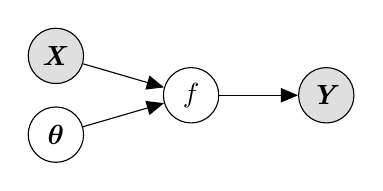
\begin{tikzpicture}
	\node[obs] (Y) {$\mat{Y}$}; %
	\node[latent, left=of Y] (f) {$f$} ; %
	\node[obs, left=of f, yshift=0.5cm] (X) {$\mat{X}$} ; %
	\node[latent, left=of f, yshift=-0.5cm] (theta) {$\bm{\theta}$} ; %
	\edge {X,theta} {f}; %
	\edge {f} {Y}; %
\end{tikzpicture}
\end{center}
\begin{itemize}
	\item Are these the assumptions? [TODO]
	\item $\mat{X}$ and $\bm{\theta}$ are independent
	\item $f$ is conditionally dependent on both $\mat{X}$ and $\bm{\theta}$
	\item $\mat{Y}$ is conditionally dependent on $f$ and conditionally independent of $\mat{X}$ and $\bm{\theta}$
\end{itemize}
\question [TODO]

There are two sources of uncertainty here, that associated with $f$ in the prior and that associated with $\epsilon$ in the likelihood, these are independent and as such are merged by simply adding to form the covariance of the marginal likelihood Gaussian.

Leaving the $\theta$ on the left-hand side of the expression [TODO]
\subsection{Practical}
\subsubsection{Linear regression}
\question [TODO]
\subsubsection{Non-parametric regression}
\question [TODO]
\question [TODO]
\section{The posterior}
\subsection{Theory}
\subsubsection{Learning}
\subsubsection{Practical optimisation}
\subsubsection{Non-parametric}
\subsection{Practical}
\subsubsection{Linear representation learning}
\end{document}
